%% TEXTE AVANCÉ %%
\section{Texte Avancé}
	\begin{frame}{Texte Avancé}
		\textbf{Que peut-on faire avec l'outil texte?}

		Une multitude de choses! Il y a une infinité de possibilités mais nous n'allons en aborder que quelques-unes.
		\begin{itemize}
			\item Projeter une ombre sous le texte
			\item Faire un texte ondulé
			\item Faire un texte en 3D
			\item Remplir du texte avec une texture ou un fond
		\end{itemize}

		On peut appliquer des filtres et des variations de couleurs à tous les textes et même les transformer en calques s'il le faut!
	\end{frame}

\begin{frame}{Texte Avancé}
	\framesubtitle{Présentation de l'outil}

	On y retrouve:
	\begin{itemize}
	\item Le choix de la police ($\rightarrow$ clic gauche sur  \inlinegraphics{Images/text/font} )
	\item La taille de la police
	\item La justification
	\item Etc
	\end{itemize}

	\begin{figure}
		\centering
		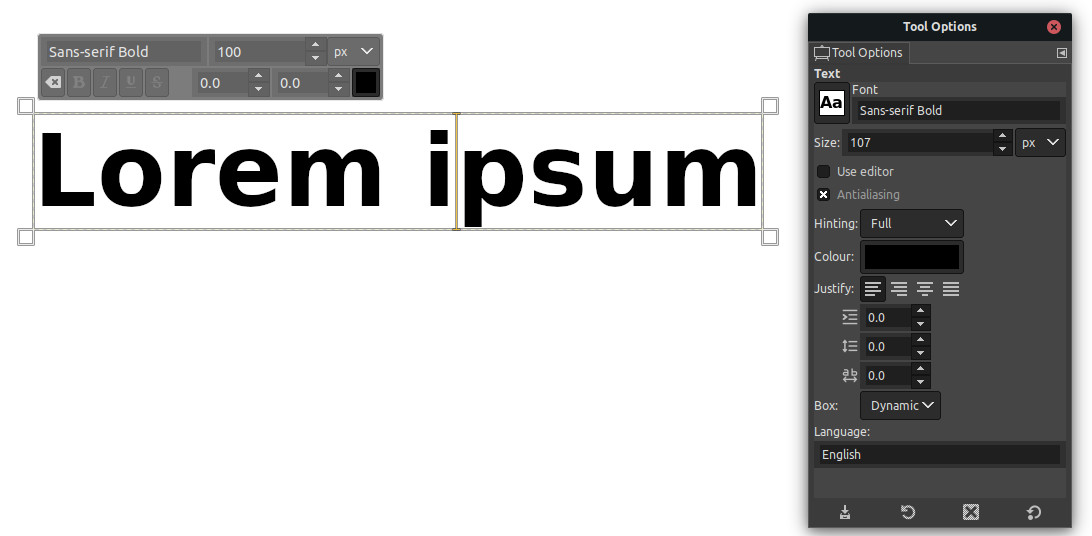
\includegraphics[height=125px]{Images/text/text}
	\end{figure}

\end{frame}



\begin{frame}{Texte Avancé}
	\framesubtitle{Ombre}
	\begin{overprint}
	\begin{itemize}
		\only<1>{
			\item[]
				\begin{figure}
				\centering
				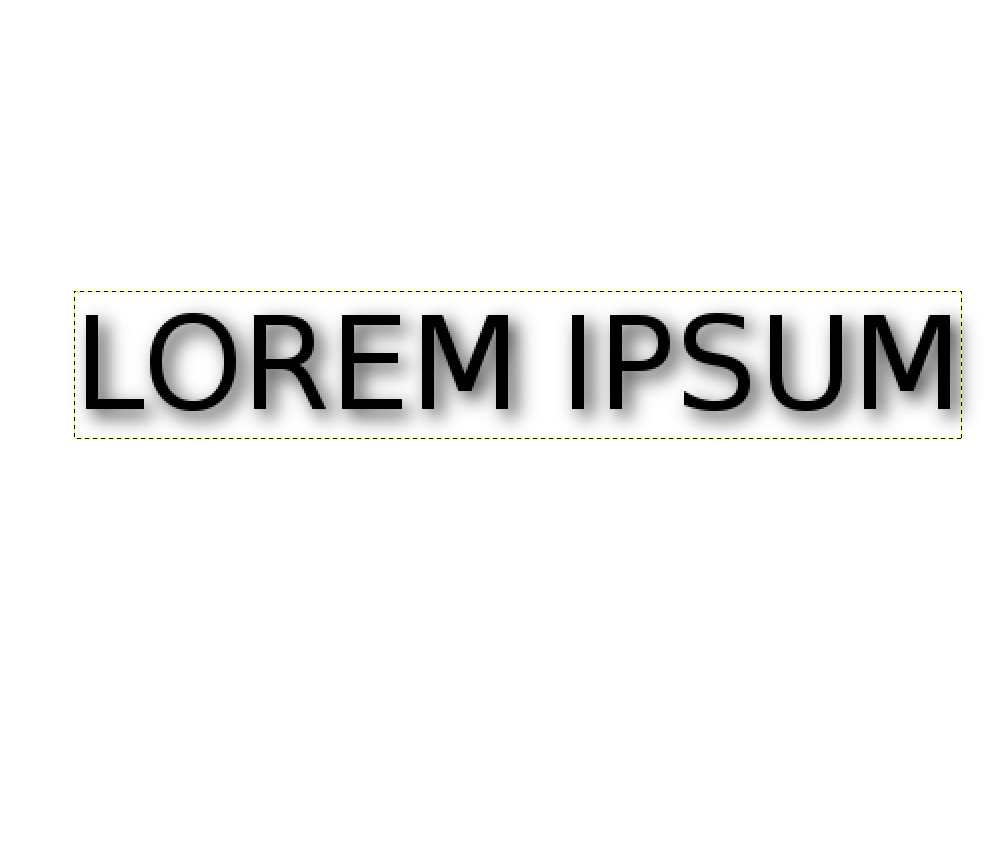
\includegraphics[height=250px]{Images/text/ombre1}
				\end{figure}
		}

		\only<2>{
			\item[]
				\textbf{Appliquer} un filtre d'ombre portée et modifier les paramètres comme on le souhaite.
				\begin{figure}
				\centering
				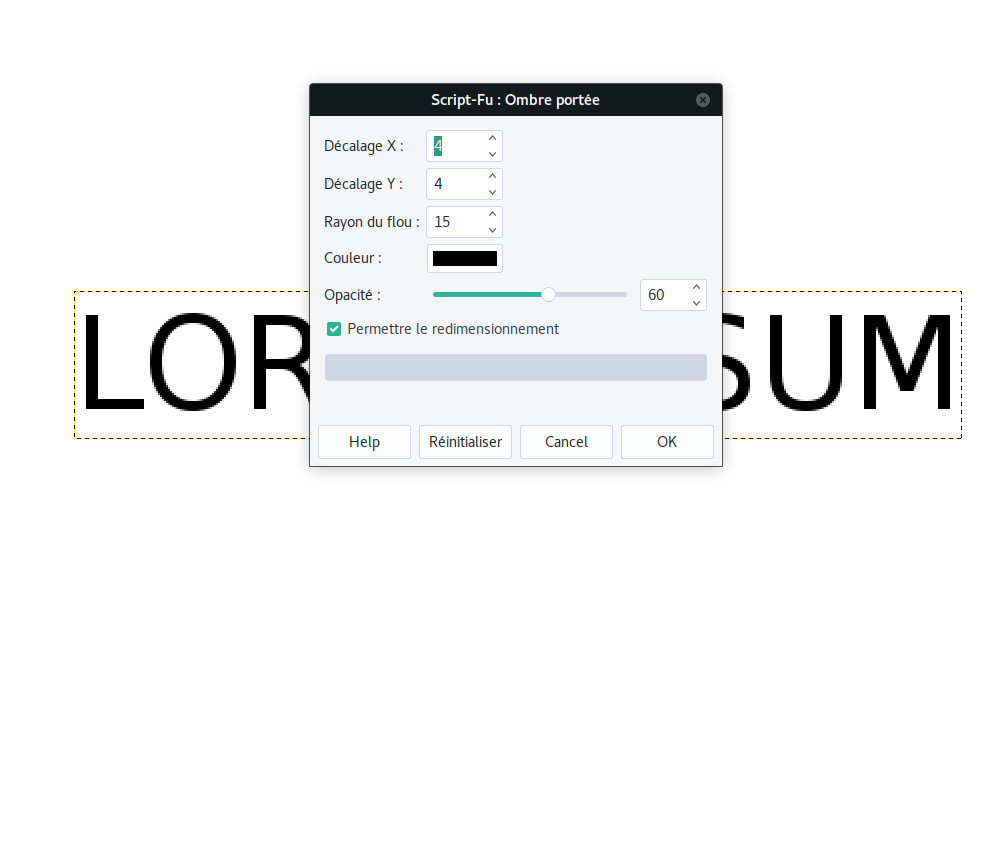
\includegraphics[height=250px]{Images/text/ombre2}
				\end{figure}
		}
		\only<3>{
			\item[]
				\textbf{Appliquer} un filtre d'ombre portée et modifier les paramètres comme on le souhaite.
				\begin{figure}
				\centering
				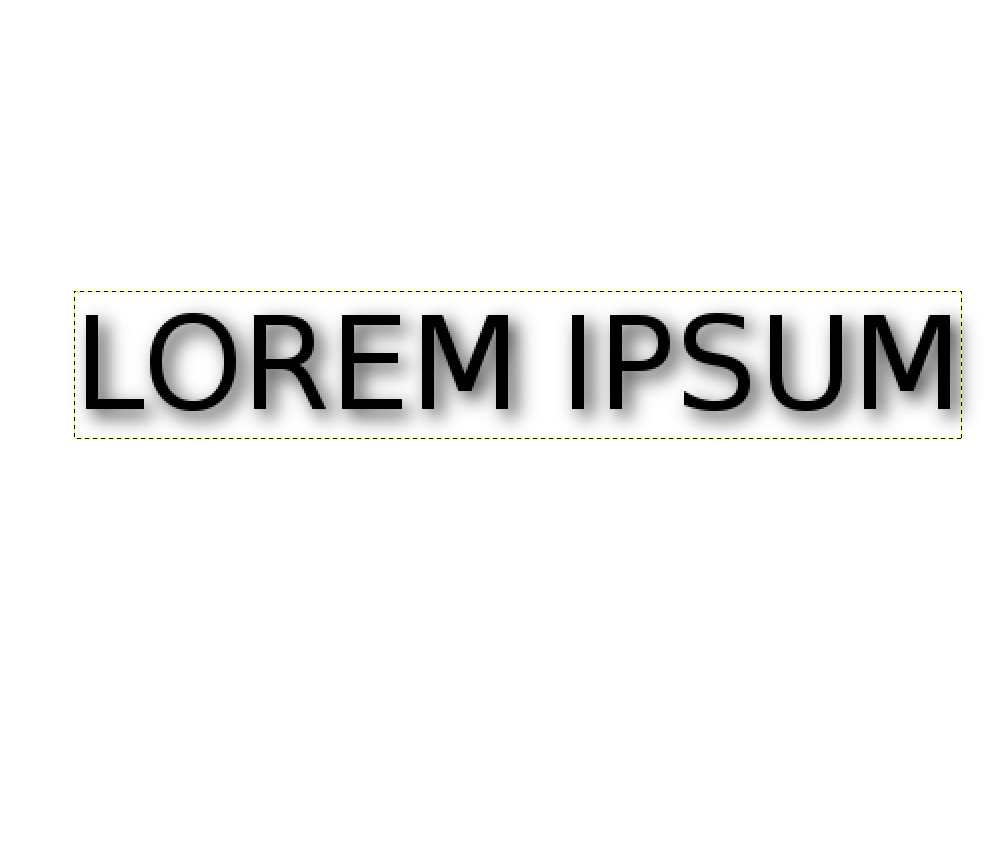
\includegraphics[height=250px]{Images/text/ombre3}
				\end{figure}
		}
	\end{itemize}
	\end{overprint}
\end{frame}

\begin{frame}{Texte Avancé}
		\framesubtitle{Texte Ondulé}
		\begin{enumerate}
			\only<1>{
				\item[]
					\begin{figure}[H]
						\centering
						\begin{minipage}{.5\textwidth}
							\centering
							
\includegraphics[height=60px]{Images/text/lorem}
							\end{minipage}$\rightarrow$%
						\begin{minipage}{.5\textwidth}
							\centering
							
\includegraphics[height=60px]{Images/text/courbf}
							\end{minipage}
					\end{figure}
			}

			\only<2>{
				\item[1.] Créer un chemin suivant le parcours désiré (touche \textbf{B}). Comme les calques, les chemins disposent de leur propre onglet et son affichables ou --par défaut-- cachés.
				\begin{figure}
					\centering
					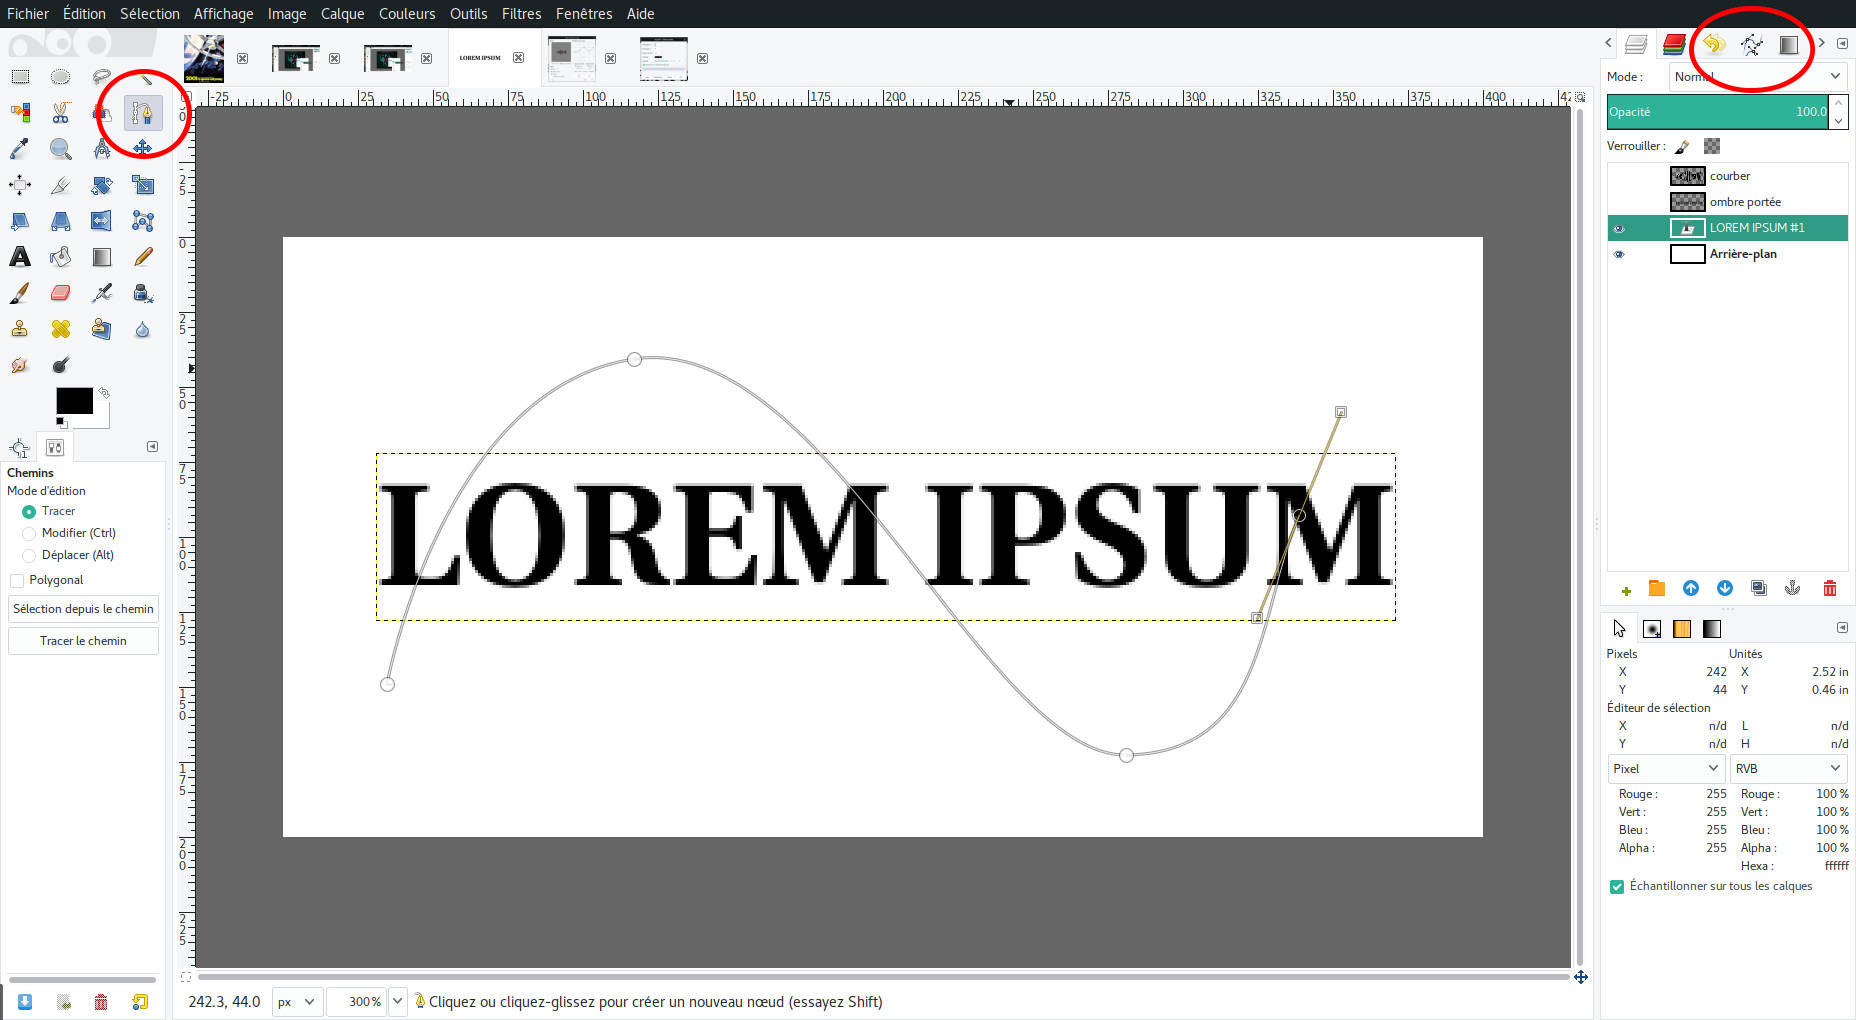
\includegraphics[height=150px]{Images/text/courb1}
				\end{figure}
			}
			\only<3>{
				\item[2.] Appliquer le texte sur le chemin (clic droit $\rightarrow$ Texte le long du chemin).
				\begin{figure}
					\centering
					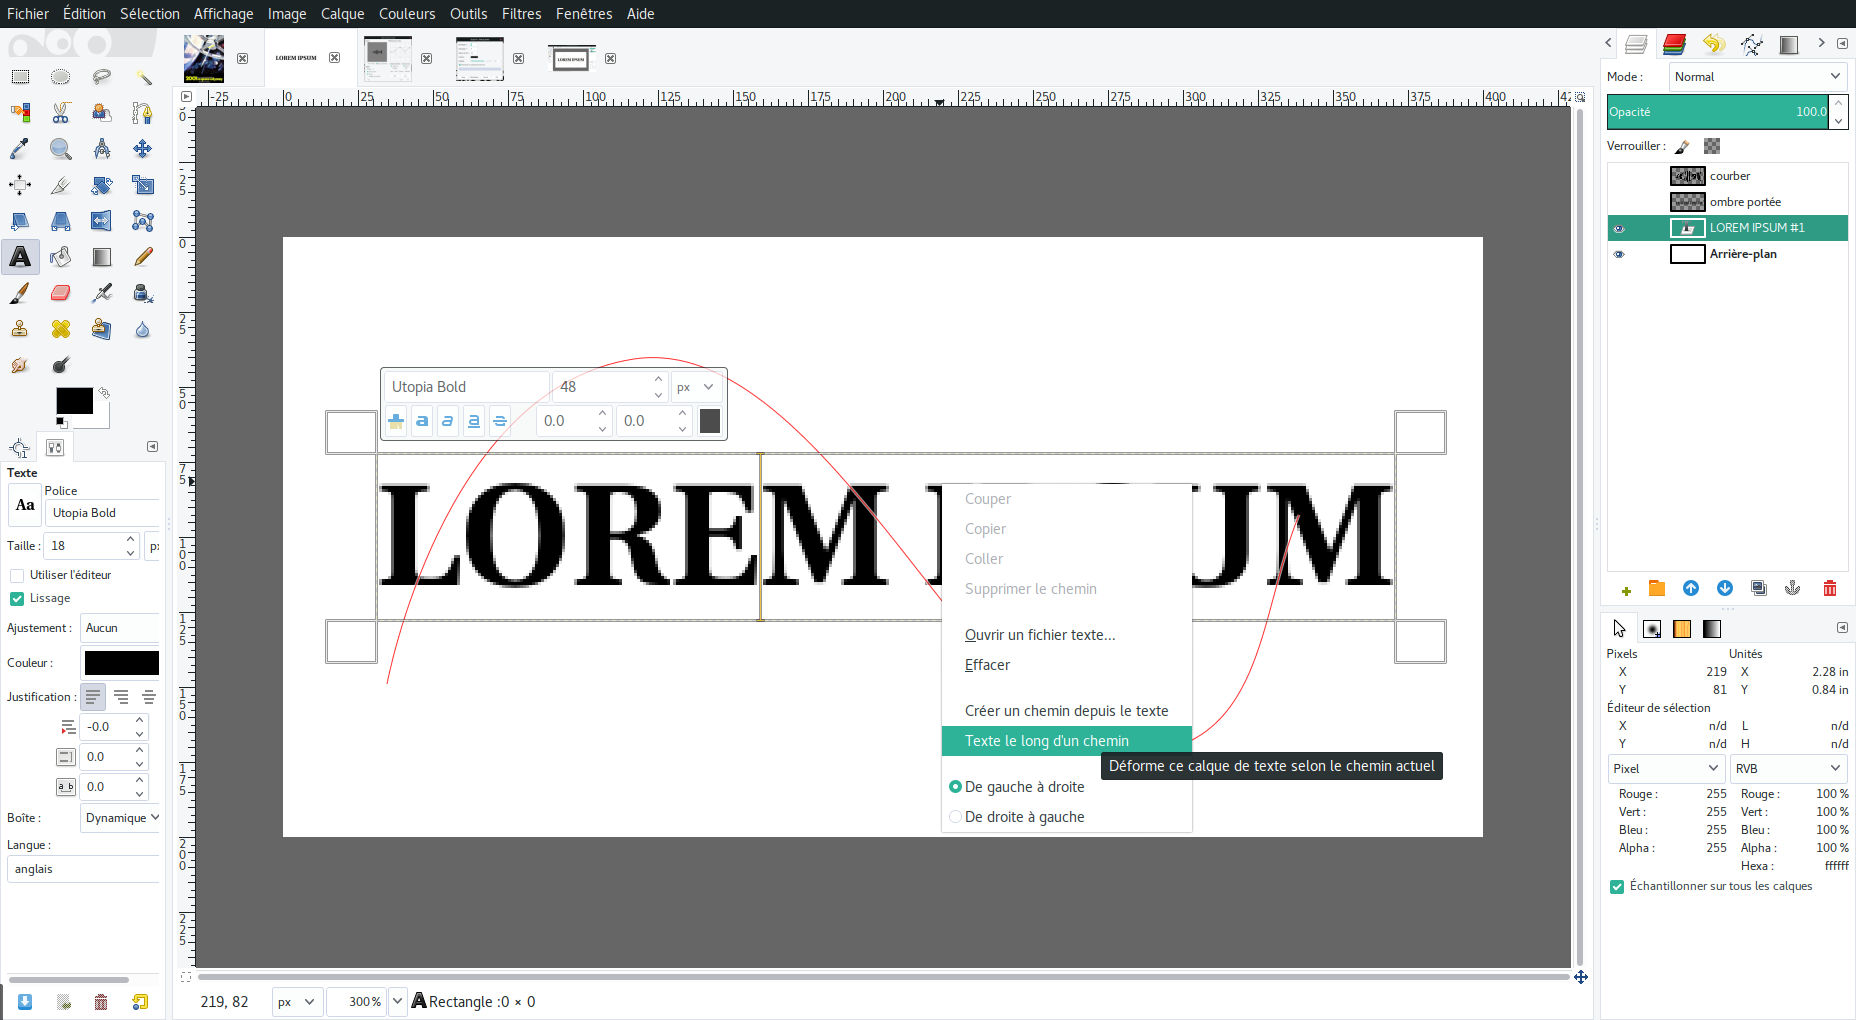
\includegraphics[height=150px]{Images/text/courb2}
				\end{figure}
			}
			\only<4>{
				\item[2.] Appliquer le texte sur le chemin (clic droit $\rightarrow$ Texte le long du chemin).
				\begin{figure}
					\centering
					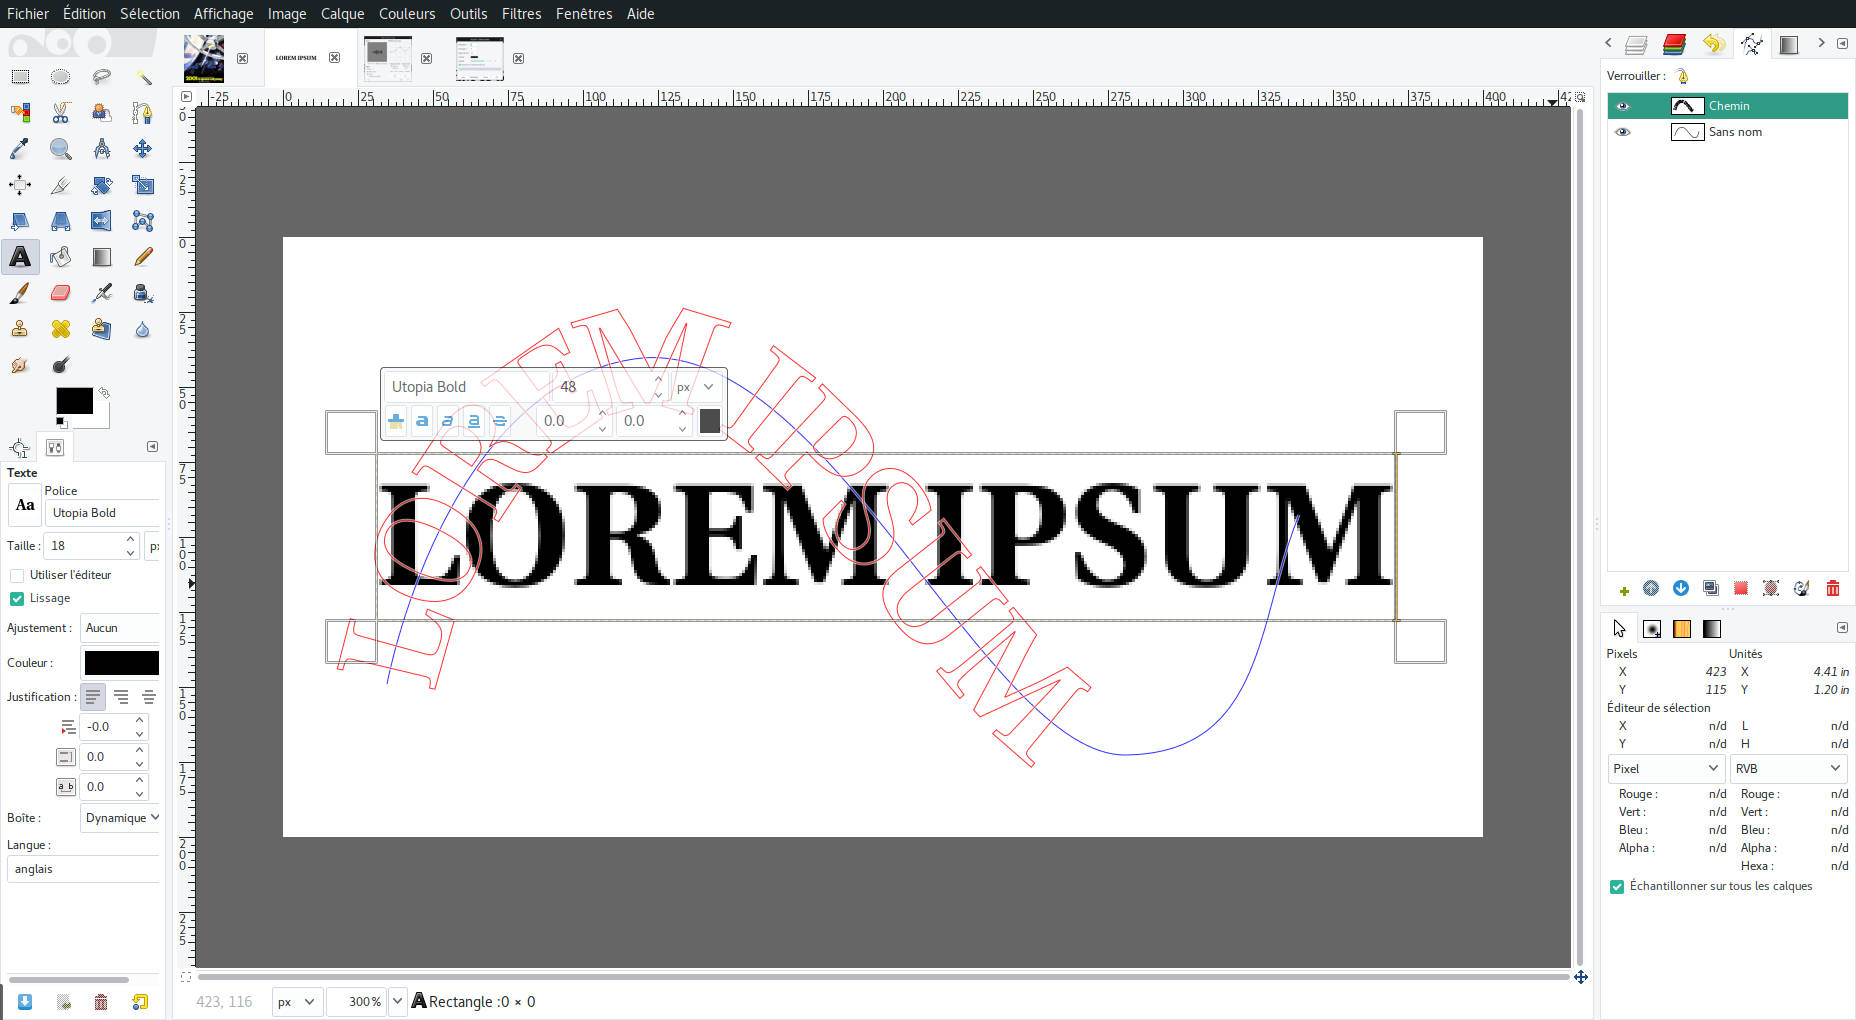
\includegraphics[height=150px]{Images/text/courb3}
				\end{figure}
			}
			\only<5>{
				\item[3.] Sélectionner le nouveau chemin et le remplir dans un nouveau calque avec la couleur voulue. 		Dans ce cas-ci, "Tracer le chemin" n'en fera que le contour ($\rightarrow$ utile pour faire une bordure sur le texte, par contre).
				\begin{figure}
					\centering
					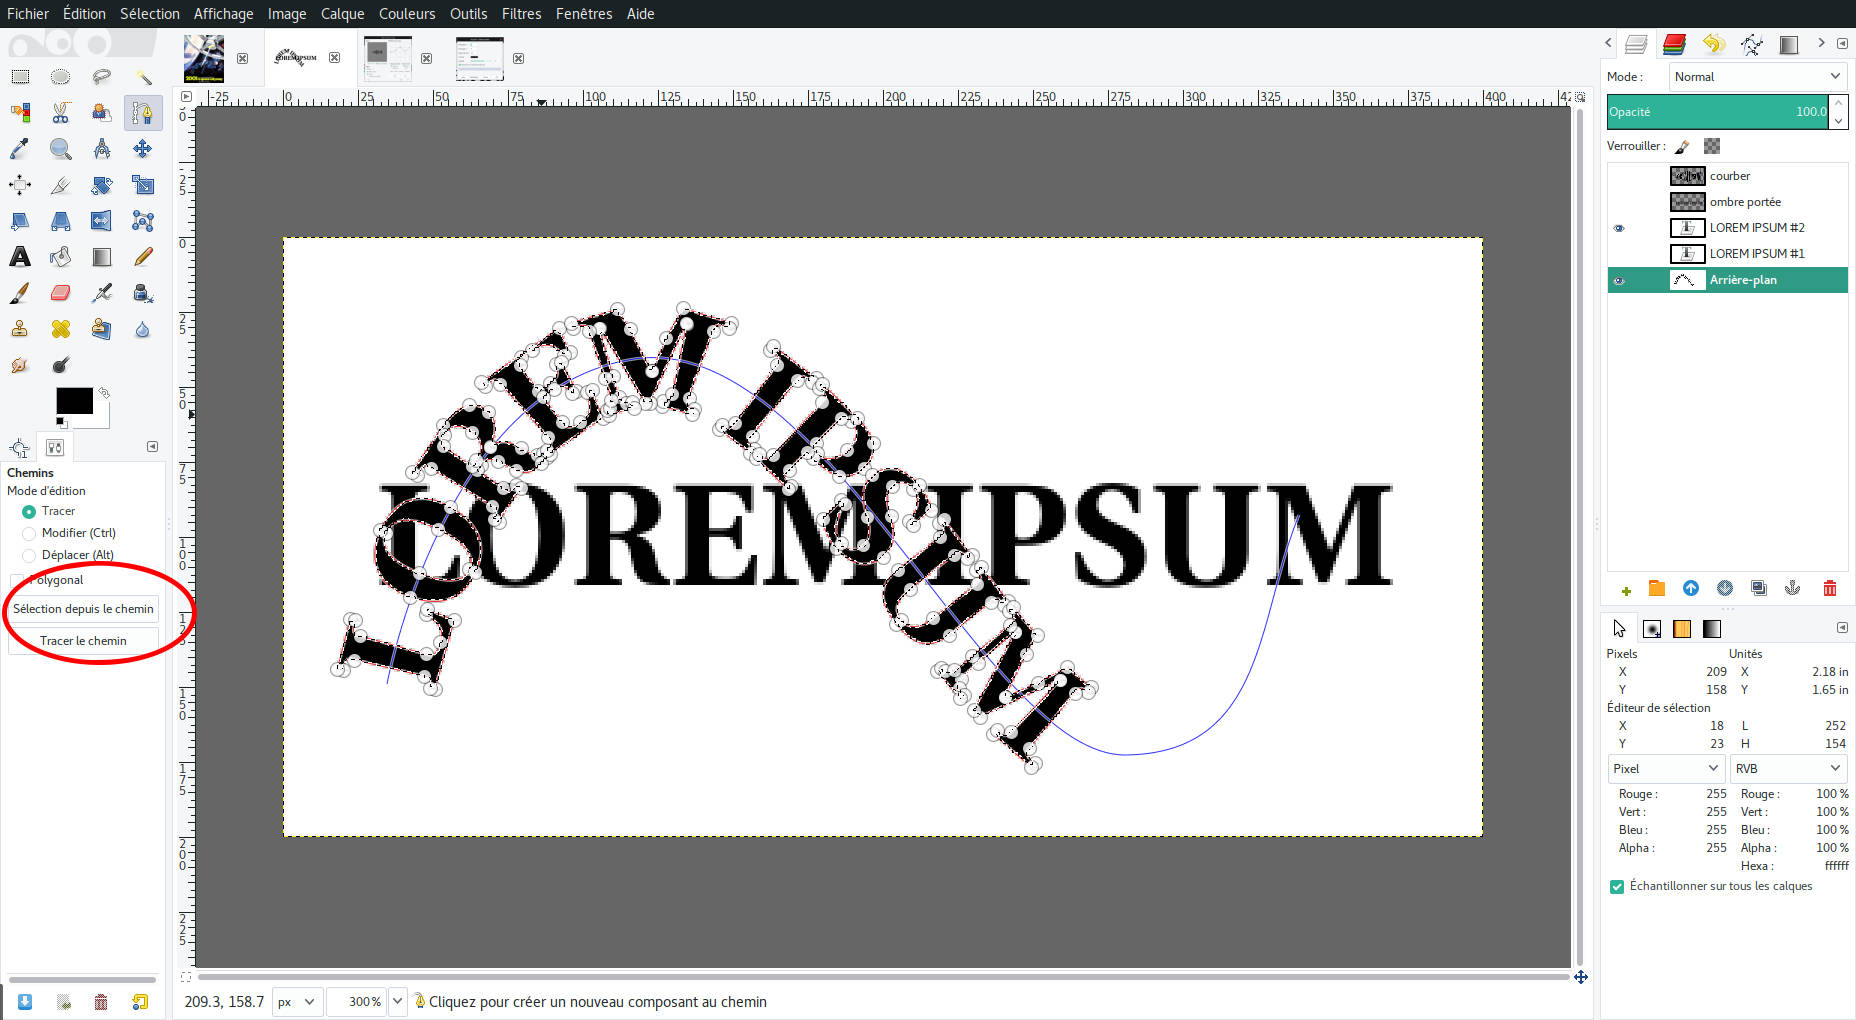
\includegraphics[height=150px]{Images/text/courb4}
				\end{figure}
			}
		\end{enumerate}
\end{frame}


\begin{frame}{Texte Avancé}
	\framesubtitle{Texte Ondulé}
	Et voilà le travail!
	\begin{figure}
	\centering
		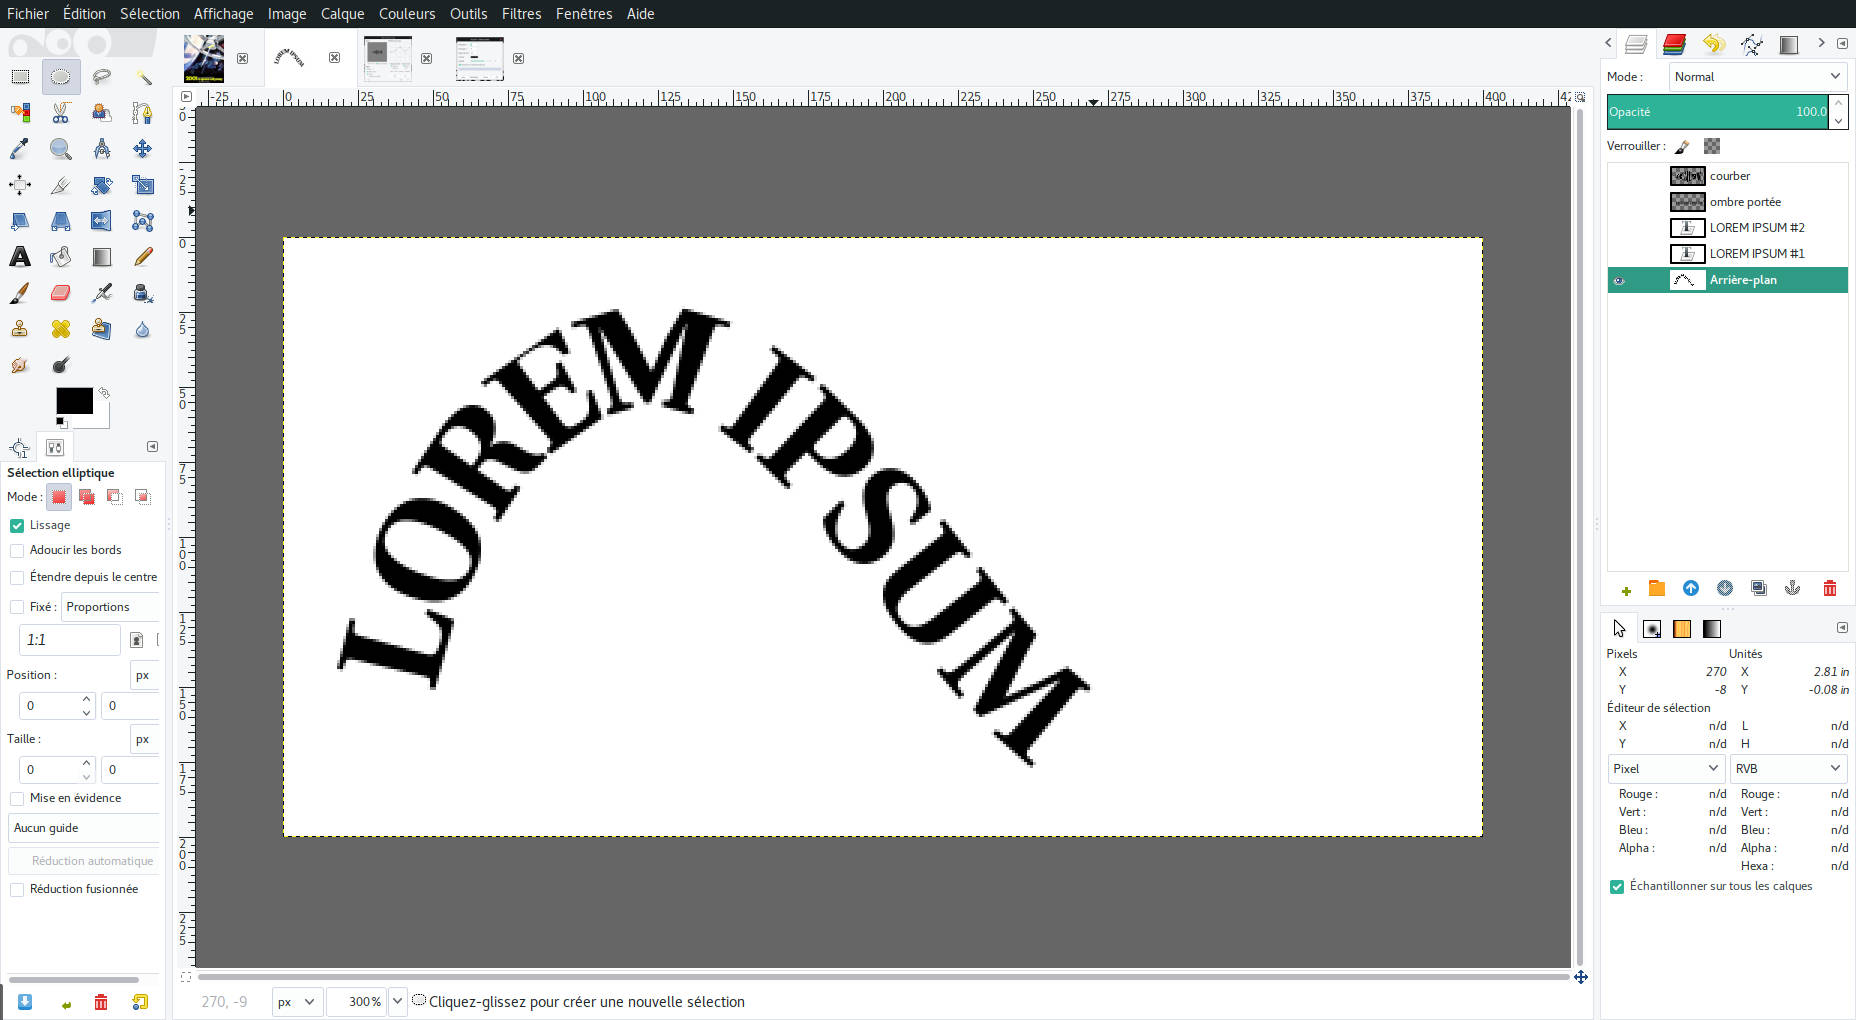
\includegraphics[height=150px]{Images/text/courb5}
	\end{figure}
\end{frame}

\begin{frame}{Texte Avancé}
	Convertir le texte en tracés est très utile pour:
	\begin{itemize}
	\item Récupérer une sélection sur base d'un texte
	\item Tracer des contours
	\item Créer une masque sur base d'un texte
	\item Transformer le texte pour le rendre plus facilement modulable
	\item Moins de risques de pertes d'informations lors de l'export vers le format pdf, par exemple
	\item Modifier une police avec l'outil éditeur de chemins
	\end{itemize}
\end{frame}


\begin{frame}{Exercice V}
\framesubtitle{Faire un meme}
	\begin{overprint}
	\begin{itemize}
		\only<1>{
			\item[]
				Image de départ: \href{http://louvainlinux.github.io/atelier-gimp/src/Images/text/meme_template.jpg}{\textcolor{webblue}{Lien de l'image}}
				\begin{figure}
					\centering
					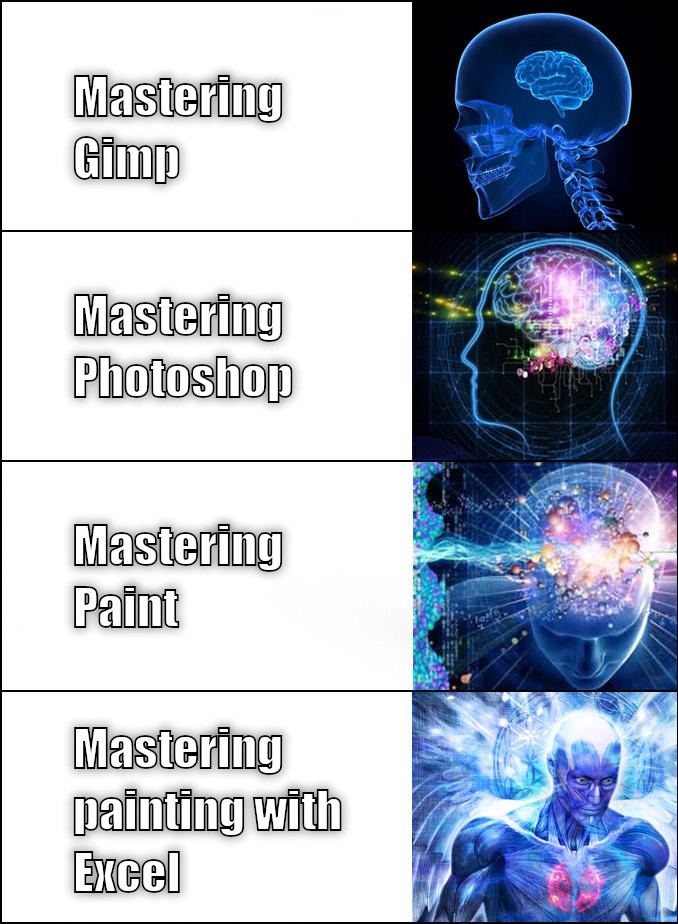
\includegraphics[height=200px]{Images/text/meme}
				\end{figure}
		}

		\only<2>{
			\item[]
				Écrire le texte.
				\begin{figure}
					\centering
					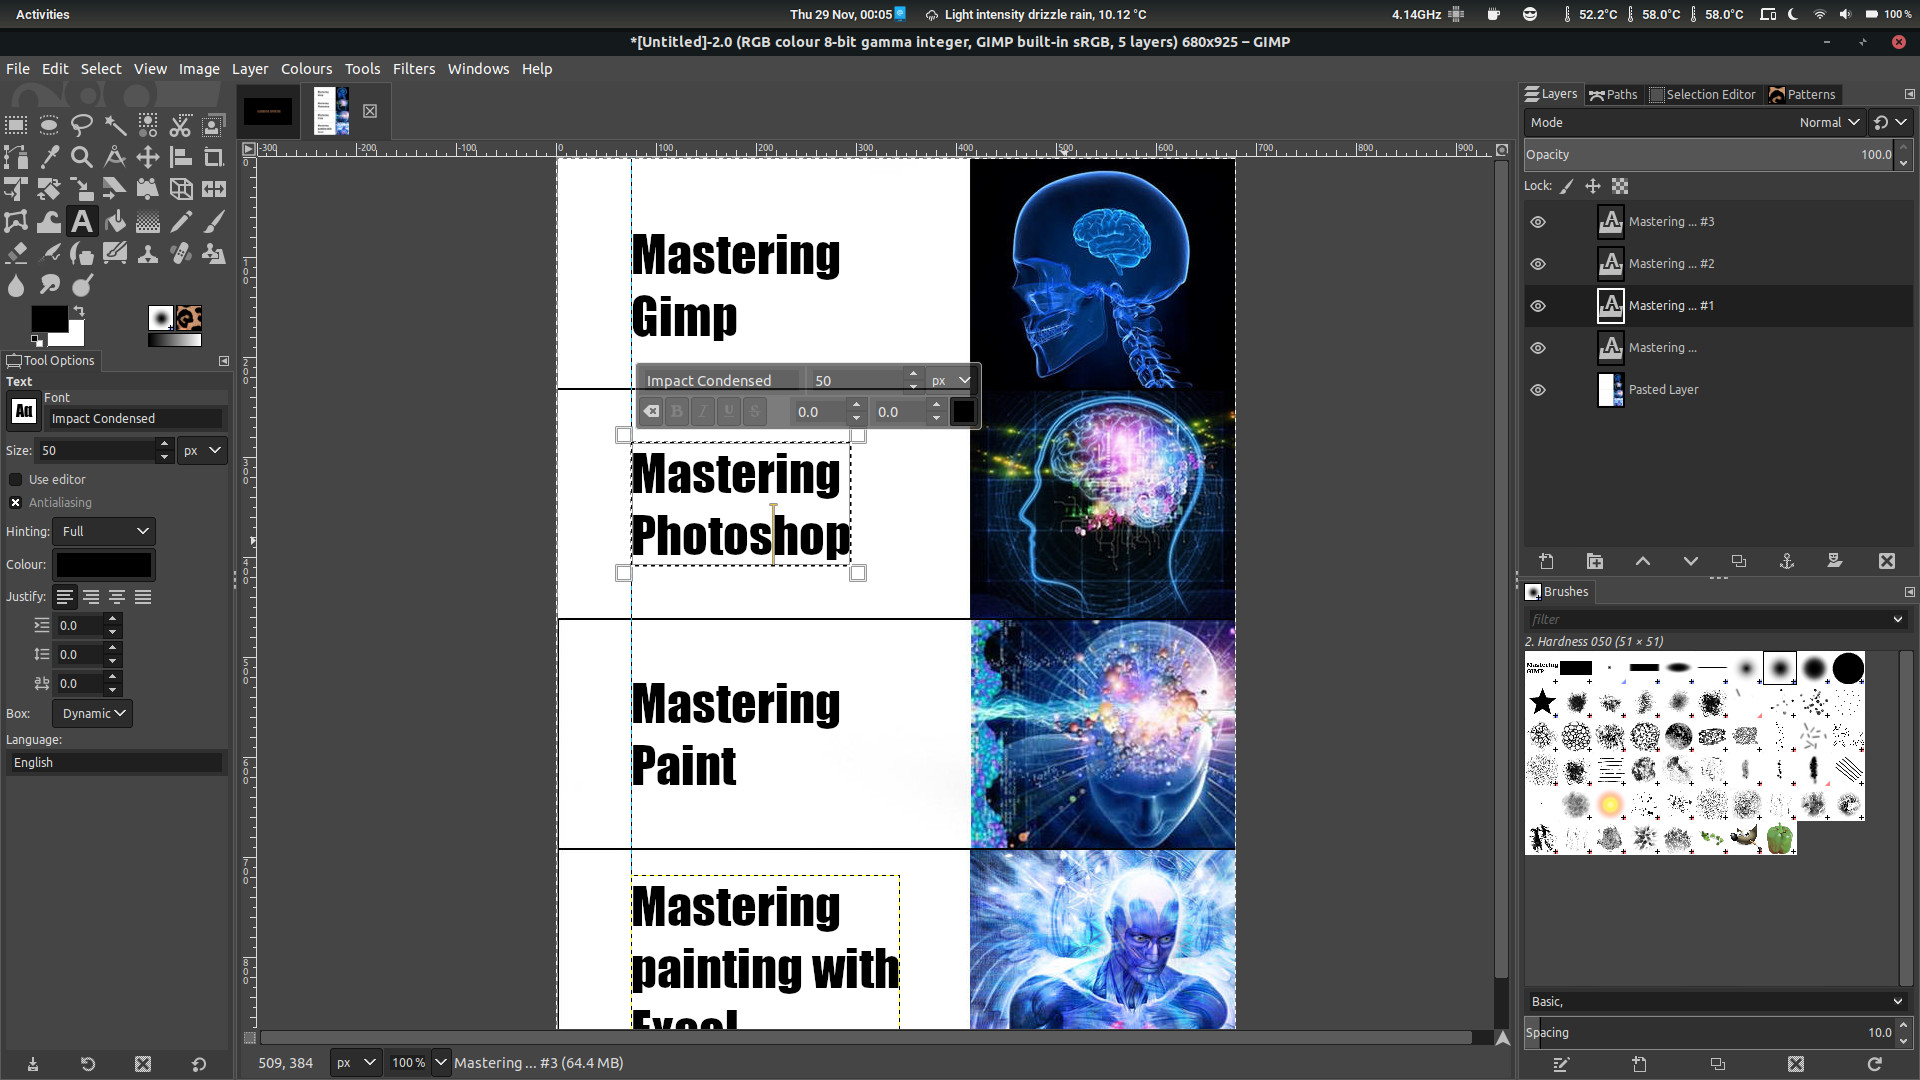
\includegraphics[width=0.90\textwidth]{Images/text/meme_txt}
				\end{figure}

		}

		\only<3>{
			\item[]
				Transformer le texte en chemin, remplir les chemins en blanc et leurs appliquer un contour noir sur un nouveau calque transparent.
				\hfill
				\begin{figure}[H]
						\centering
						\begin{minipage}{.5\textwidth}
							\centering
							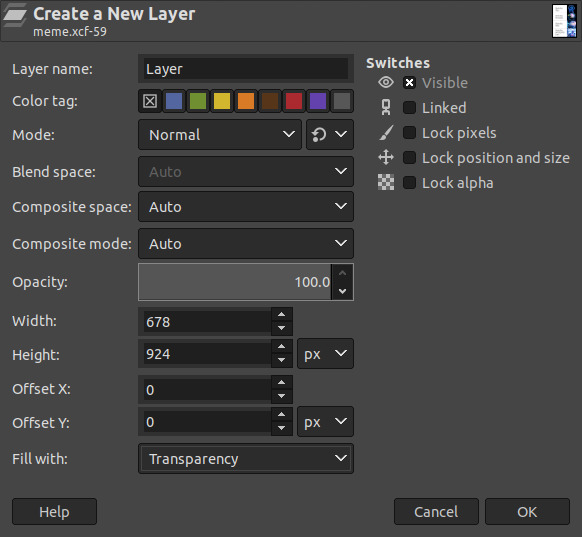
\includegraphics[width=0.90\textwidth]{Images/text/new_layer}
							\end{minipage}%
						\begin{minipage}{.5\textwidth}
							\centering
							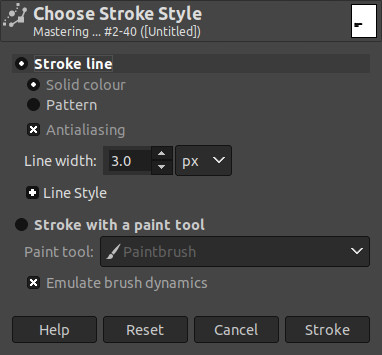
\includegraphics[width=0.90\textwidth]{Images/text/stroke_style}
							\end{minipage}
					\end{figure}
		}
	\end{itemize}
	\end{overprint}
\end{frame}
